\section{背景}
  \frame
  {
    \frametitle{\secname~ }
    \begin{block}{凸包围体技术}
      在计算机图形学领域里的各种算法中发挥着重要作用,
      如优化渲染和建模过程,加速求交、碰撞检测等算法。
    \end{block}
    \begin{block}{碰撞检测问题}
   计算机图形学、虚拟现实等领域中的研究热点,
   是计算机模拟真实环境中不可或缺的技术,
   在物理仿真及游戏领域里应用十分广泛。
    \end{block}
    \note{
      凸包围体技术在计算机图形学领域里的各种算法中发挥着重要作用,如优化渲染和建模过程,加速求交、碰撞检测等算法。
      主要是用在原始模型之间的相关计算(遮挡测试、相交测试等)之前进行预处理判断和剪枝,以求交算法为例,如果两个模型相交,则对应的凸包围体一定相交,
      若凸包围体不相交则其对应的原始模型一定不相交。而一般来讲,判断凸包围体是否相交比判断原始模型相交更简单,因此可以提升效率。
      
      碰撞检测问题是计算机图形学、虚拟现实等领域中的研究热点,是计算机模拟真实环境中不可或缺的技术,在物理仿真及游戏领域里应用十分广泛。
      例如在游戏中,碰撞检测技术增强了游戏的真实性,游戏中的角色行走不可穿墙、角色中弹而亡等等都离不开碰撞检测技术。
    }
  }

  \subsection{凸包围体}
  \frame{
  \frametitle{凸包围体的种类}
  \begin{figure}
  \hspace{-2.0em}
    \begin{minipage}{1.06\textwidth}
    \subfloat[\scriptsize AABB]
        {
           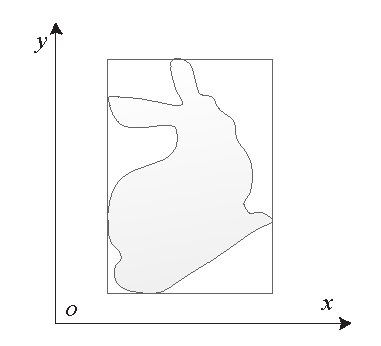
\includegraphics[width=0.2\textwidth]{figures/bunny-2d-AABB.eps}
        }
        \subfloat[\scriptsize OBB]
        {
            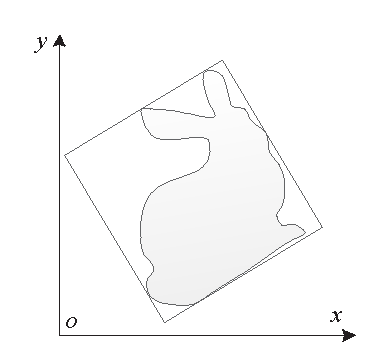
\includegraphics[width=0.2\textwidth]{figures/bunny-2d-OBB.eps}
        }
       \subfloat[\scriptsize Sphere]
        {
           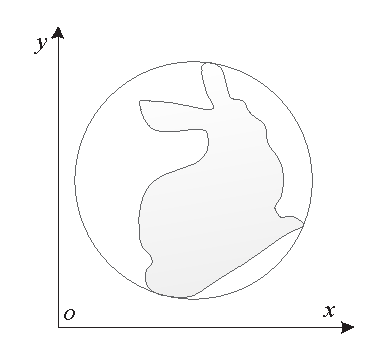
\includegraphics[width=0.2\textwidth]{figures/bunny-2d-Sphere.eps}
        }%\linebreak
        \subfloat[\scriptsize $k$-DOP]
        {
           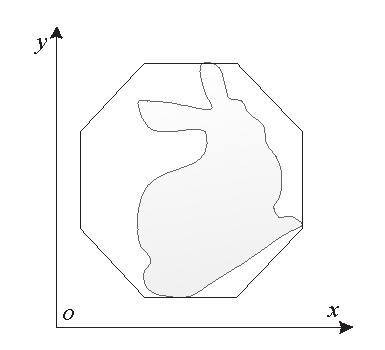
\includegraphics[width=0.2\textwidth]{figures/bunny-2d-8DOP.eps}
        }
        \subfloat[\scriptsize 凸包]
        {
           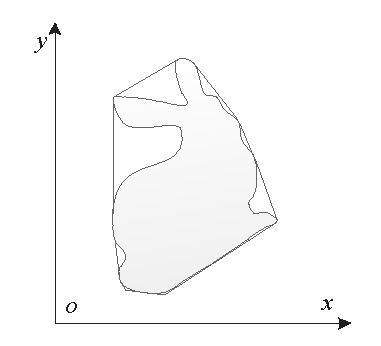
\includegraphics[width=0.2\textwidth]{figures/bunny-2d-Convexhull.eps}
        }
        \end{minipage}
        \caption{不同种类的包围体}
        \label{chart:exps:tightness}
        \end{figure}
        \vspace{-1em}
      其他:Tribox、Swept-sphere、 Sphere-shell、Zonotopes、圆柱形、圆锥、椭球形等等。
      
      \note{
        上面这几个就是最常见的凸包围体。最常见的沿坐标轴方向的AABB包围盒,带方向的包围盒OBB,包围球,k面的凸包围体(k-DOP),和凸包,还有一些比较特定领域用的圆柱、圆锥形、椭球形等等。
        其中k-DOP是采用k/2对固定方向的半空间相交构成的凸包围体,是综合比较较好的包围体,因为可以通过k来调节包围体的简单性和紧致性来满足不同应用的需求。
      }
  }

      \frame{
   \frametitle{本文目标}
     \footnotesize
     \textbf{$k$-DOP}\footfullcite{klosowski1998efficient}的局限性:方向\textbf{固定}且为\textbf{有限的偶数},不同模型其截面方向一致, \textbf{不够紧致};\\ 
     而凸包很(最)紧致,但面片数量太多,构造复杂度$O(n\log n)$。
    \begin{block}{本文凸包围体的目标}
      \hspace{-2.0em}   \begin{minipage}{\textwidth}
    \begin{description}
      \item[紧致:] 能够自适应模型,根据模型形状特点有不同的方向;
      \item[快速:] 生成凸包围体的速度要快,利用~GPU~加速;
      \item[灵活:] 通过参数~$k$~调节凸包围体的简单性和紧致程度。
    \end{description}
  \end{minipage}
    \end{block}

       \note{
         描述PPT。
本文提出的 k-CBP 与 k-DOP 不同之处在于:
(1) k-DOP 中 k 值通常仅局限于少数几个,例如 k = 6,8,14,18,20,26 等,后面那篇文
献最大支持 k = 46),且 k-DOP 中方向是成对平行的,k 值是偶数,而 k-CBP 中
的 k 理论上可以是任意的,奇偶都可以;
(2) k-DOP 中的凸多面体方向是固定的即 k 值确定之后,不管输入模型的点集
分布如何, k-DOP 的方向始终保持一致,本文则提出了一种能够自适应模型的算
法使得构造的凸包围多面体足够紧致;
(3) k-CBP 中 k 取值灵活,必须找出一种算法生成 k 个法向,比只有少数几个可直接通过枚举方向的 k-DOP 取值更复杂。
通过更加紧致的 k-CBP 去近似原始模型,能够达到更好的精度,且输入 k 值
可以自由控制,为其能够用于碰撞检测等应用提供足够大的灵活性。
       }
  }

  \subsection{碰撞检测算法}
   \frame{
   \frametitle{\subsecname~ }
    
   \begin{block}{碰撞检测算法}
     许多应用的基础,例如在~3D~游戏,物理仿真,机器人,虚拟现实等领域中\footfullcite{ericson2005real}。
   \end{block}

   \begin{block}{分类}
     \begin{description}
       \item[加速结构:] SPT(如四叉树、KD~树等)~v.s~\textbf{BVH}(OBB树、$k$-DOP树等)
       \item[表现形式:] \textbf{刚体}~v.s~可变形,凸体~v.s~凹体,CSG~v.s~参数曲面~v.s~\textbf{多边形网格}
       \item[碰撞环境:] \textbf{成对}~v.s~\textbf{多体},\textbf{静止}~v.s~\textbf{运动},\textbf{离散}~v.s~连续
     \end{description}
   \end{block}
   
   \note{
    (介绍PPT后),本文后面的实验就是基于BVH的,不可变形的三角网格。//现在研究较多的是连续的可变形的碰撞检测布料模拟头发模拟等。
   }
  }

  \frame{
    \frametitle{基于~BVH~的碰撞检测算法}
    \begin{columns}[onlytextwidth]
      \begin{column}{0.35\textwidth}
        \vspace{-1.5em}
        \begin{figure}[htbp]
            \begin{center}
            \begin{boxedminipage}{1\textwidth}
            \subfloat{\label{lbl:bvh-bunny-center-0.png}}
              {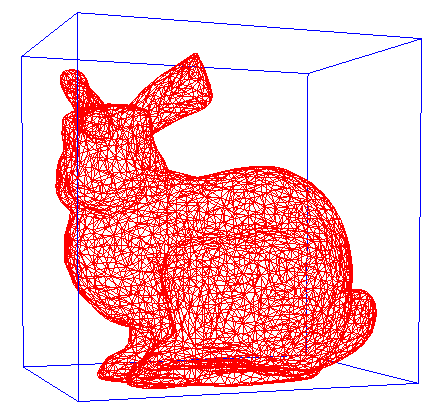
\includegraphics[height=1.4cm]{bvh-bunny-center-0.png}}
            \subfloat{\label{lbl:bvh-bunny-center-1.png}}
              {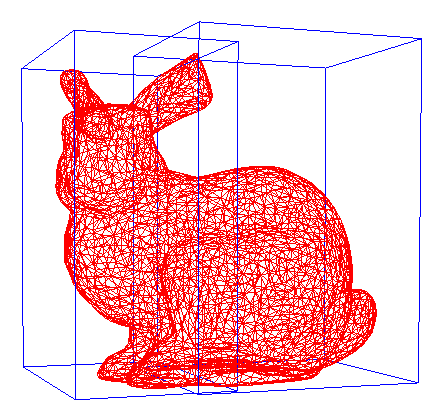
\includegraphics[height=1.4cm]{bvh-bunny-center-1.png}}
            \\
            \subfloat{\label{lbl:bvh-bunny-center-2.png}}
              {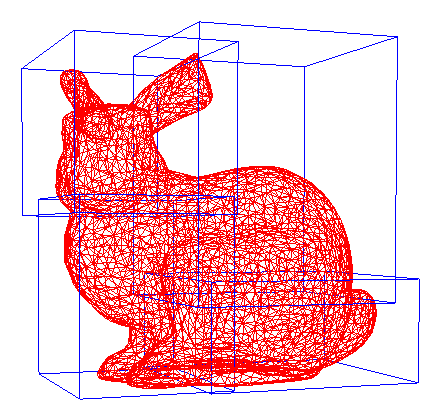
\includegraphics[height=1.4cm]{bvh-bunny-center-2.png}}
            \subfloat{\label{lbl:bvh-bunny-center-3.png}}
              {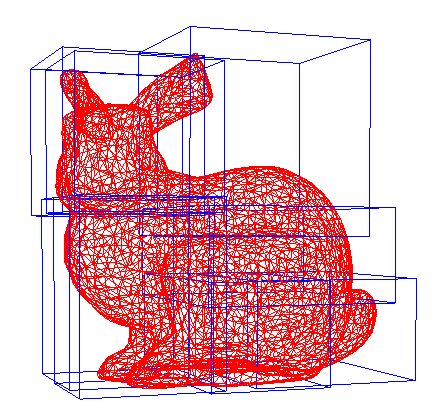
\includegraphics[height=1.4cm]{bvh-bunny-center-3.png}}
            \\\hspace{0.5cm}
            \subfloat{\label{lbl:bvh-bunny-center-4.png}}
              {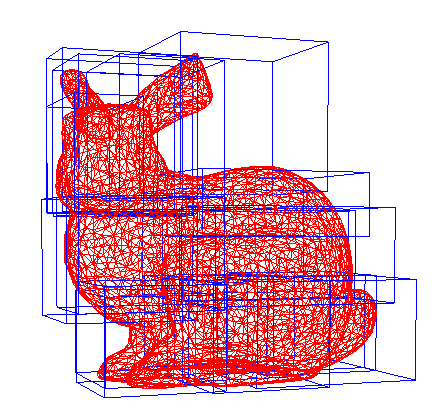
\includegraphics[height=1.5cm]{bvh-bunny-center-4.png}}
            \subfloat{\label{lbl:bvh-bunny-center-5.png}}
              {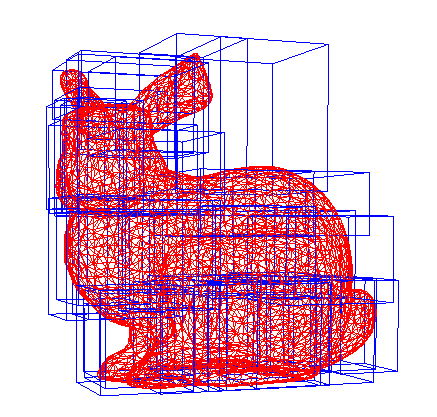
\includegraphics[height=1.5cm]{bvh-bunny-center-5.png}}
            \\
            \subfloat{\label{lbl:bvh-bunny-center-6.png}}
              {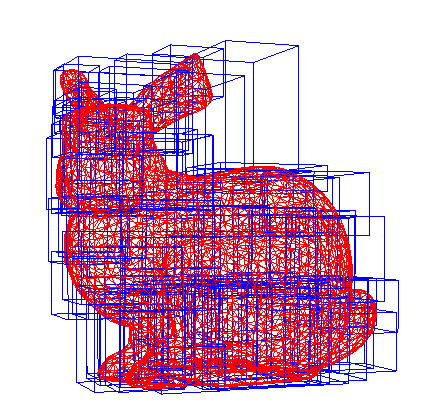
\includegraphics[height=1.5cm]{bvh-bunny-center-6.png}}
            \subfloat{\label{lbl:bvh-bunny-center-7.png}}
              {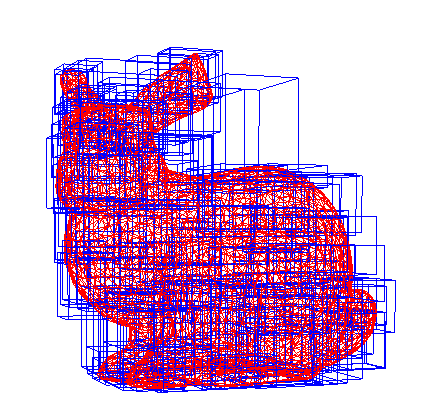
\includegraphics[height=1.5cm]{bvh-bunny-center-7.png}}
            \end{boxedminipage}
            \vspace{-0.5em}
          \caption{八层~BVH~示例}
          \label{lbl:bvh-example}
          \end{center}
          \end{figure}
      \end{column}
      \hspace{0.5em}
      \begin{column}{1.2\textwidth}
      \vspace{0.2em}
         \scalebox{0.5}{
              \begin{minipage}{1.0\textwidth}
      \vspace{-2em}
           \begin{algorithm}[H]
              \caption{自顶向下层次遍历~BVH~}
              \label{alg:traverse-bvh-tree}
              \begin{algorithmic}[1]
              \Require
              两个~BVH~树的根节点~$node_1$,$node_2$
              \Ensure
              模型是否相交
              \Function {TraverseBVHTree}{$node_1, node_2$}
                \If{$node_1.bv \cap node_2.bv = \emptyset$}
                  \State \Return{\textbf{False}}
                  \Comment{包围体重合测试, 包围体不相交直接返回}
                \Else
                    \If {$node_1.children = \emptyset$}
                         \If {$node_2.children = \emptyset$}
                         \State \Comment{最底层叶子节点原生几何相交测试}
                         \State \Return {\Call{CheckIntersection}{$node_1.primitives, node_2.primitives$}}
                         \Else
                            \ForAll {$child \in node_2.children$}
                            \State \Call{TraverseBVHTree}{$node_1, child$} \Comment{递归调用}
                            \EndFor
                         \EndIf
                    \Else
                         \ForAll {$child \in node_1.children$}
                         \State \Call{TraverseBVHTree}{$child, node_2$}  \Comment{递归调用}
                         \EndFor
                    \EndIf
                \EndIf
              \EndFunction
              \end{algorithmic}
              \end{algorithm}
              \end{minipage}
            }
      \\
      \scriptsize \hspace{1em}代价函数: $T_{cost} = n_v * C_v + n_p * C_p + (n_u * C_u)$(运动)
      \end{column}
    \end{columns}
    \note{
      基于包围体树的碰撞检测算法, 一般首先都会初始化环境然后构建层次结构的包围体树,碰撞检测时从顶层开始逐渐往下层遍历,到最底层叶子节点后开始三角网格模型相交测试,
      当发现三角网格相交后立即终止遍历,确定模型发生碰撞。
      评价碰撞检测算法的指标一般用上面这个公式来衡量,其中nv和 np分别表示参与包围体节点相交测试的数量和参与原始几何相交测试的数量,Cv和 Cp则表示相应的平均测试耗费的代价。
      当在运动场景时还需要加上nu和 Cn就是模型旋转或者运动后包围体更新的数量和更新的代价。
      本文算法就是尽早发现包围体不相交的情况,减少np和cp的数量。
    }
}
